%%%%%%%%%%%%%%%%%%%%%%%%%%%%%%%%%%%%%%%%%
% Beamer Presentation
% LaTeX Template
% Version 1.0 (10/11/12)
%
% This template has been downloaded from:
% http://www.LaTeXTemplates.com
%
% License:
% CC BY-NC-SA 3.0 (http://creativecommons.org/licenses/by-nc-sa/3.0/)
%
%%%%%%%%%%%%%%%%%%%%%%%%%%%%%%%%%%%%%%%%%

%----------------------------------------------------------------------------------------
%	PACKAGES AND THEMES
%----------------------------------------------------------------------------------------

\documentclass[10pt]{beamer}
\mode<presentation> {

% The Beamer class comes with a number of default slide themes
% which change the colors and layouts of slides. Below this is a list
% of all the themes, uncomment each in turn to see what they look like.

%\usetheme{default}
%\usetheme{AnnArbor}
%\usetheme{Antibes}
%\usetheme{Bergen}
%\usetheme{Berkeley}����JFIF����C
%\usetheme{Berlin}
%\usetheme{Boadilla}
%\usetheme{CambridgeUS}
%\usetheme{Copenhagen}
%\usetheme{Darmstadt}
%\usetheme{Dresden}
%\usetheme{Frankfurt}
%\usetheme{Goettingen}
%\usetheme{Hannover}
%\usetheme{Ilmenau}
%\usetheme{JuanLesPins}
%\usetheme{Luebeck}
%\usetheme{Madrid}
%\usetheme{Malmoe}
%\usetheme{Marburg}
%\usetheme{Montpellier}
\usetheme{PaloAlto}
%\usetheme{Pittsburgh}
%\usetheme{Rochester}
%\usetheme{Singapore}
%\usetheme{Szeged}
%\usetheme{Warsaw}

% As well as themes, the Beamer class has a number of color themes
% for any slide theme. Uncomment each of these in turn to see how it
% changes the colors of your current slide theme.

%\usecolortheme{albatross}
%\usecolortheme{beaver}
%\usecolortheme{beetle}
%\usecolortheme{crane}
%\usecolortheme{dolphin}
%\usecolortheme{dove}
%\usecolortheme{fly}
%\usecolortheme{lily}
%\usecolortheme{orchid}
%\usecolortheme{rose}
%\usecolortheme{seagull}
%\usecolortheme{seahorse}
\usecolortheme{whale}
%\usecolortheme{wolverine}

%\setbeamertemplate{footline} % To remove the footer line in all slides uncomment this line
\setbeamertemplate{footline}[page number] % To replace the footer line in all slides with a simple slide count uncomment this line

%\setbeamertemplate{navigation symbols}{} % To remove the navigation symbols from the bottom of all slides uncomment this line
}

\usepackage{graphicx} % Allows including images
\usepackage{booktabs} % Allows the use of \toprule, \midrule and \bottomrule in tables
\usepackage{amsmath}
\usepackage{subfig}
\usepackage{caption}
\usepackage{mathabx}
\usepackage{wasysym}
\usepackage{wrapfig}
\usepackage{tikz}
\usepackage{animate}
\usepackage{minted}
\usepackage{listings}
\usepackage{listings}
\usetikzlibrary{shapes.geometric, arrows}
\usepackage{minted}
\usepackage{color}

\usepackage{xcolor}
\usepackage{listings}
\lstset{basicstyle=\ttfamily,
  showstringspaces=false,
  commentstyle=\color{red},
  keywordstyle=\color{blue}
}

%\usepackage{subcaption}
%----------------------------------------------------------------------------------------
%	TITLE PAGE
%----------------------------------------------------------------------------------------
\title[]{Lab \#4: WiFi Pineapple \\ Wi-Fi deauthentication attack \\  } % The short title appears at the bottom of every slide, the full title is only on the title page

\author{Alexander Blaauwgeers} % Your name
\institute[University of Amsterdam] % Your institution as it will appear on the bottom of every slide, may be shorthand to save space
{
University of Amsterdam \\ % Your institution for the title page
\medskip
%\textit{john@smith.com} % Your email address
}
\date{Mei 16, 2018} % Date, can be changed to a custom date

\begin{document}

\begin{frame}
\titlepage % Print the title page as the first slide
\end{frame}

%----------------------------------------------------------------------------------
% \section{Introduction }
% \begin{frame}{Introduction}
% \begin{block}{Question}
% There are radio stations that send out RDS information so you know traffic jams are ahead or know the name of the
% song that is currently playing.
% \begin{itemize}
%     \item Is there a way to retrieve this information using SDR?
%     \item What kind of information can you get out of this?
%     \item How does the protocol work?
% \end{itemize}
% \end{block}
% \end{frame}

\begin{frame}{Questions}

\begin{itemize}
    \item What can you do with the WiFi Pineapple?
    \item What is a Wi-Fi deauthentication attack?
    \item Can you preform an Wi-Fi deauthentication attack?
\end{itemize}

\begin{itemize}
    \item How do you get the information? Probes?
    \item Scenarios for an Wi-Fi deauthentication attack?
    \item Can you use a Wi-Fi deauthentication attack as stepping stone?
\end{itemize}
\end{frame}

%----------------------------------------------------------------------------------
\section{Theory}
%----------------------------------------------------------------------------------
\begin{frame}{Theory - The concept behind the attack}
\centering
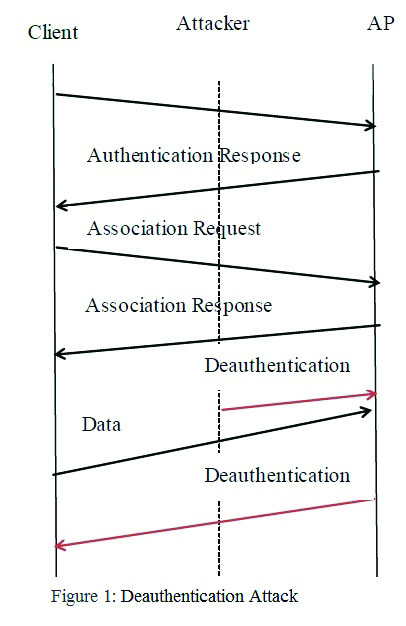
\includegraphics[width=135px]{dewifi.jpg}\footnote{\tiny{https://opensourceforu.com/2015/04/beware-it\%C2\%92s-easy-to-launch-a-wireless-deauthentication-attack/}}

\end{frame}

%----------------------------------------------------------------------------------
\section{Networks and associations}
%----------------------------------------------------------------------------------
\begin{frame}{Networks and associations}
\centering
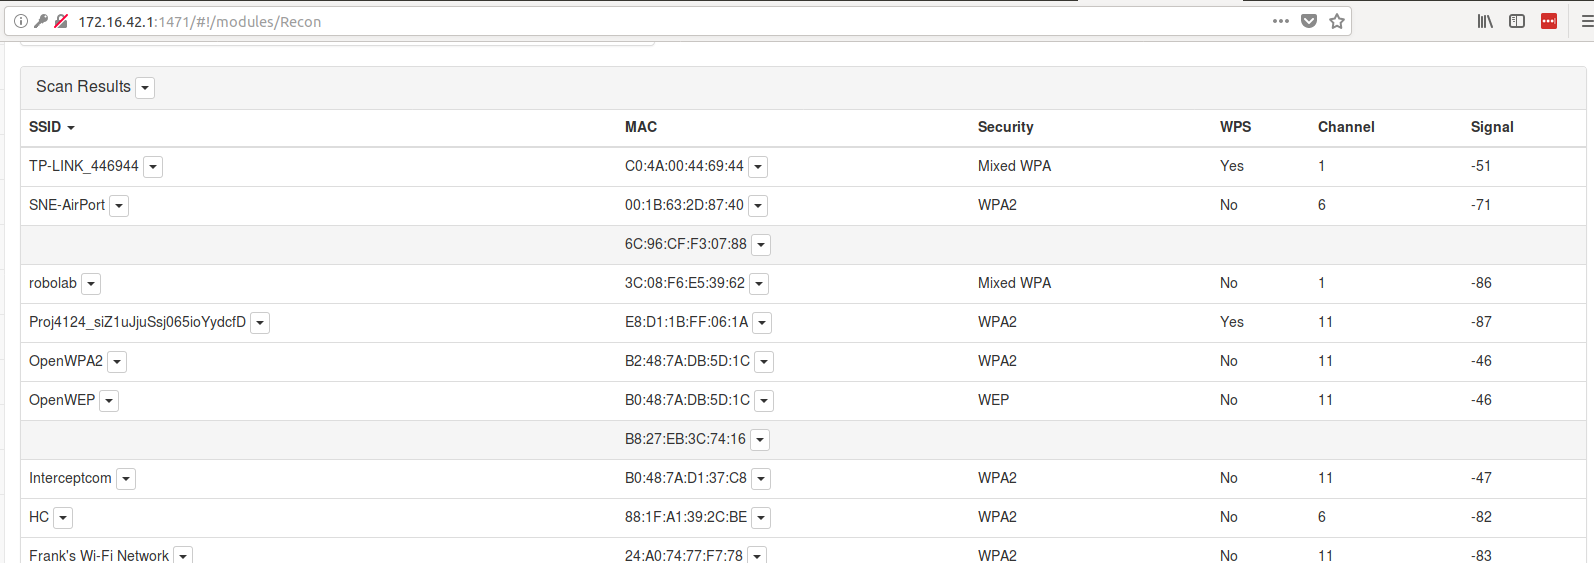
\includegraphics[width=\textwidth]{recon1.png}
\end{frame}

\begin{frame}{Networks and associations}
\centering
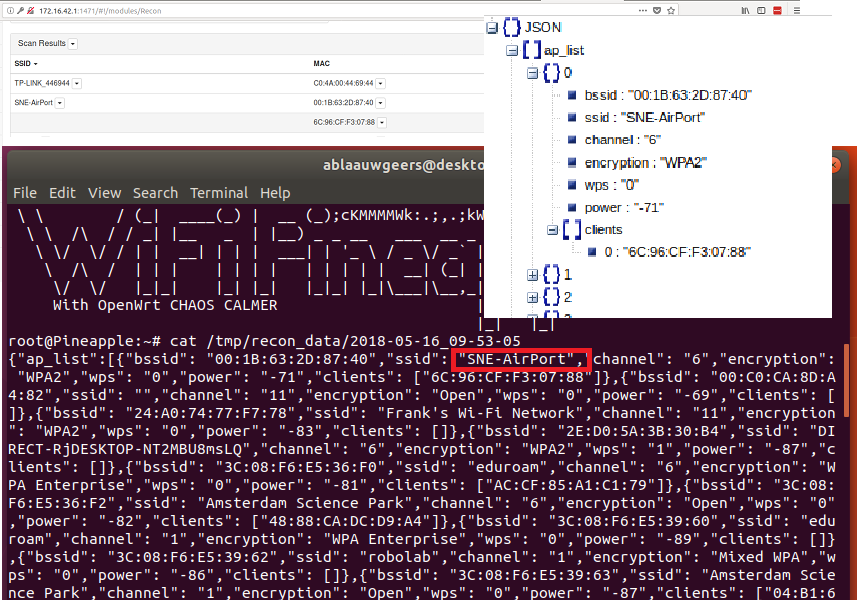
\includegraphics[width=\textwidth]{JSONx.png}
\end{frame}

%----------------------------------------------------------------------------------
\section{Probe}
%----------------------------------------------------------------------------------
\begin{frame}{Probe}
\centering
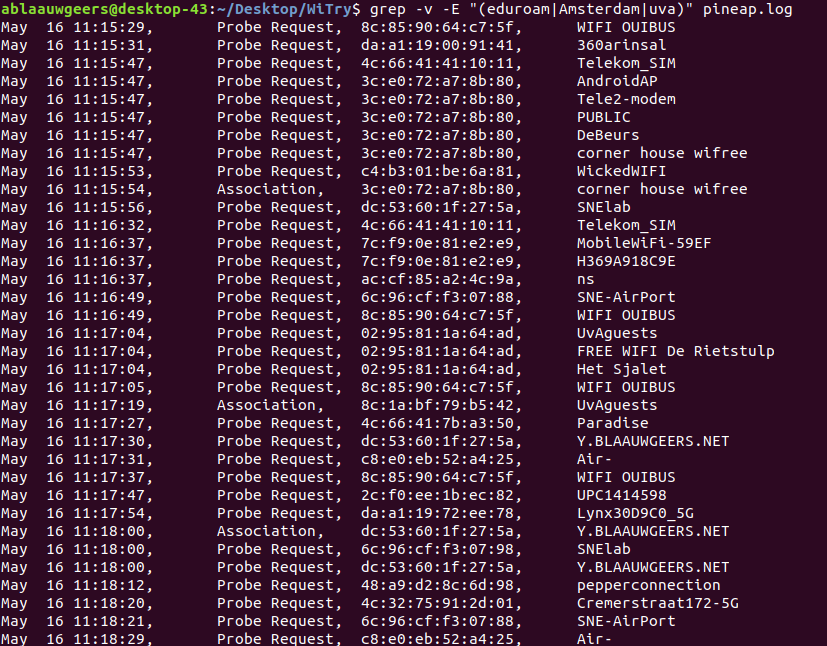
\includegraphics[width=\textwidth]{probe.png}
\end{frame}

\begin{frame}{Probe Zoom}
\centering
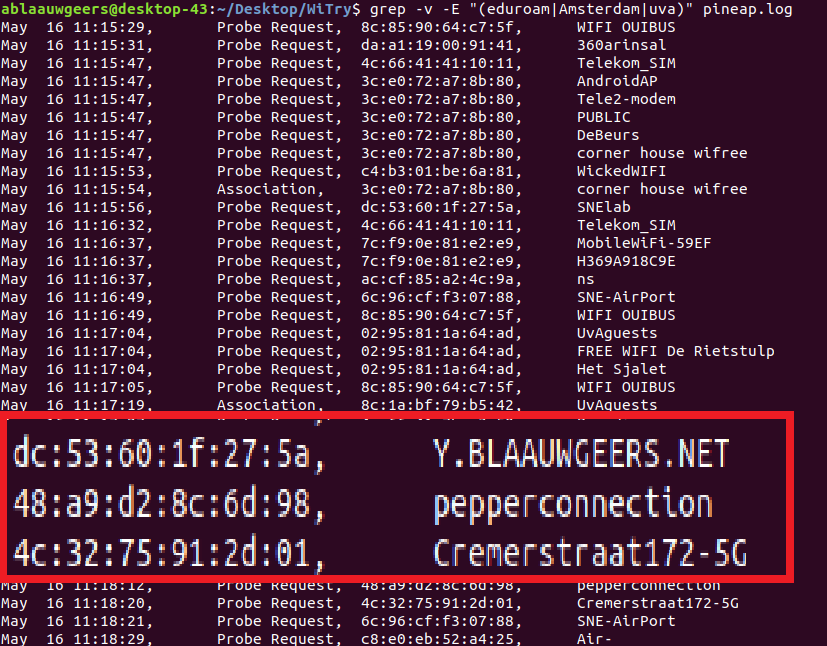
\includegraphics[width=\textwidth]{probe2.png}
\end{frame}

\begin{frame}{Probe Social Engineering}
\centering
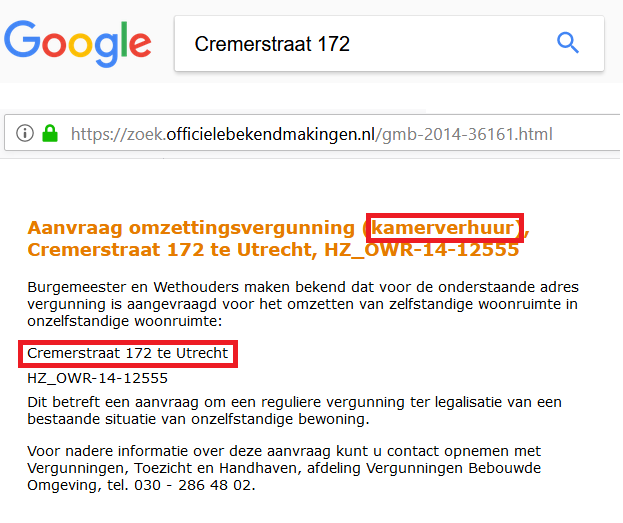
\includegraphics[width=\textwidth]{omzet.png}
\end{frame}

%----------------------------------------------------------------------------------
\section{Wi-Fi deauthentication attack}
%----------------------------------------------------------------------------------
\begin{frame}{Back to the deauthentication}
\centering
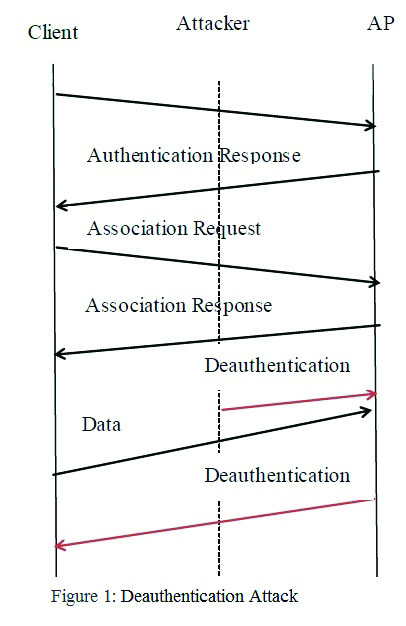
\includegraphics[width=100px]{dewifi.jpg}\footnote{\tiny{https://opensourceforu.com/2015/04/beware-it\%C2\%92s-easy-to-launch-a-wireless-deauthentication-attack/}}
\end{frame}

\begin{frame}{What can you do? MitM}
\centering
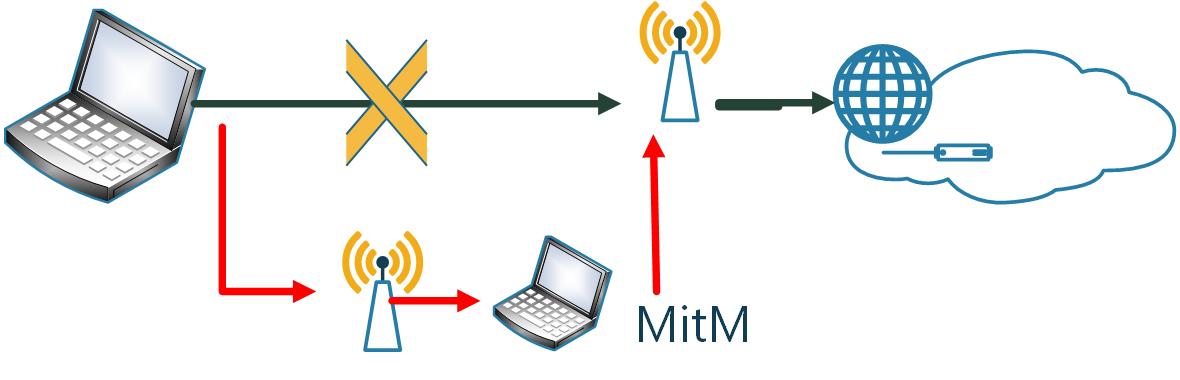
\includegraphics[width=\textwidth]{MinM.png}
\end{frame}

\begin{frame}{What can you do? Break hotspot}
\centering
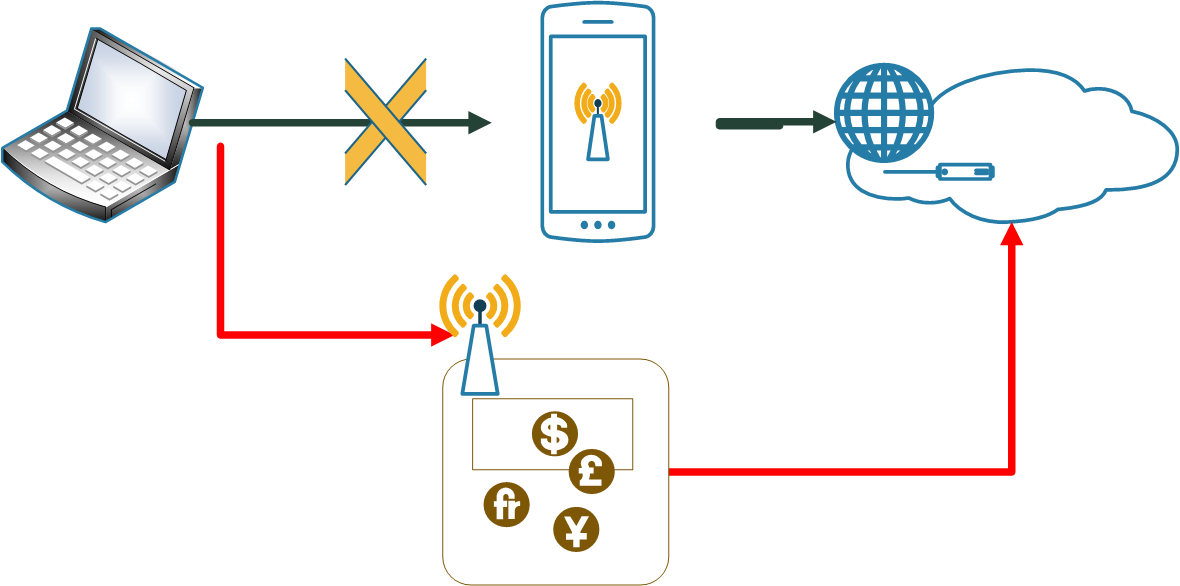
\includegraphics[width=\textwidth]{hotel.png}
\end{frame}

%----------------------------------------------------------------------------------
\section{News}
%----------------------------------------------------------------------------------

\begin{frame}{News}
\centering
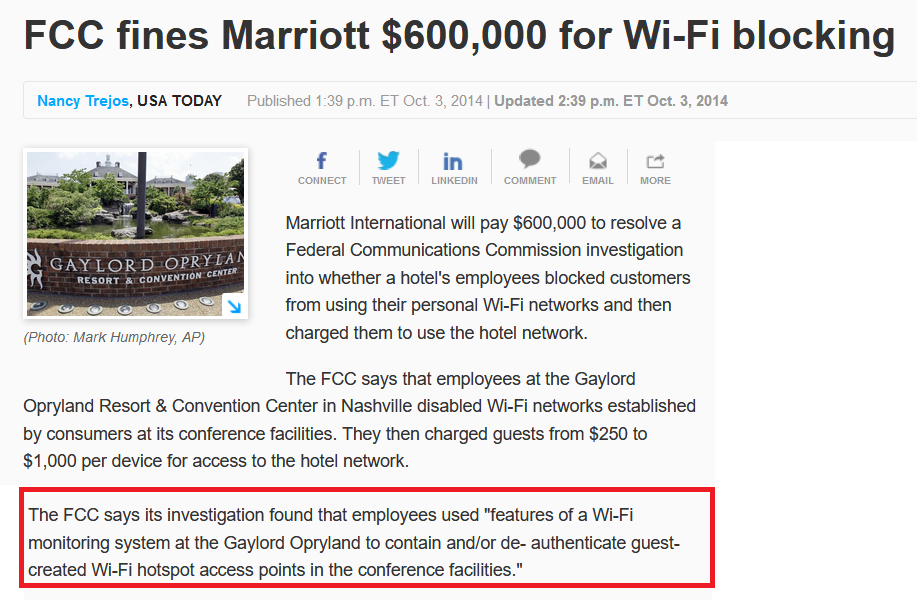
\includegraphics[width=\textwidth]{hotelfcc.png}\footnote{\tine{https://www.usatoday.com/story/money/business/2014/10/03/marriott-fcc-nashville-fined-wifi-blocking/16648695/}}
\end{frame}

%----------------------------------------------------------------------------------
\section{PoC MitM attack}
%----------------------------------------------------------------------------------

\begin{frame}{Wi-Fi deauthentication}
\centering
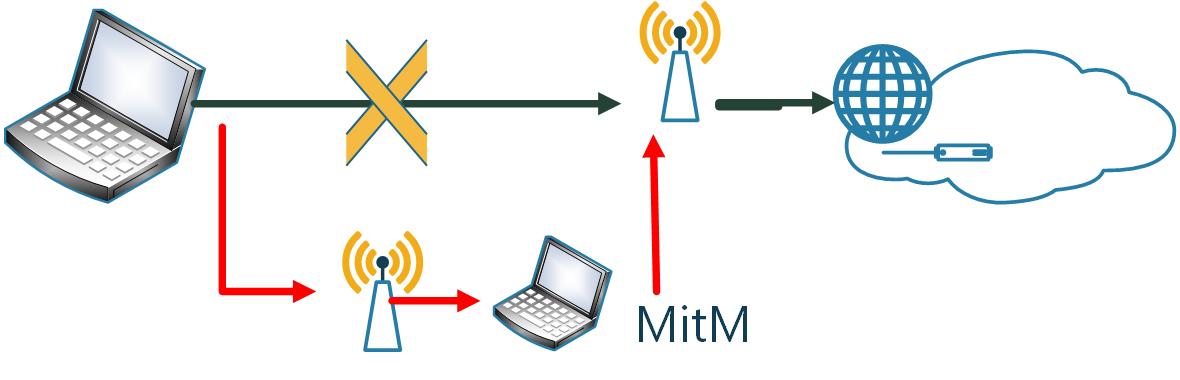
\includegraphics[width=\textwidth]{MinM.png}\\
aireplay-ng -0 10 -a 40:4E:36:CC:18:A9 -c DC:53:60:1F:27:5A wlan0\\
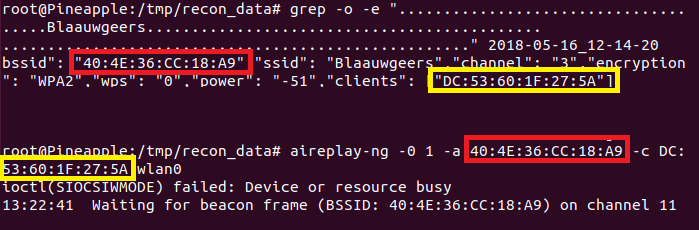
\includegraphics[width=\textwidth]{codedauth.png}
\end{frame}



\begin{frame}{Wi-Fi MitM attack}
\centering
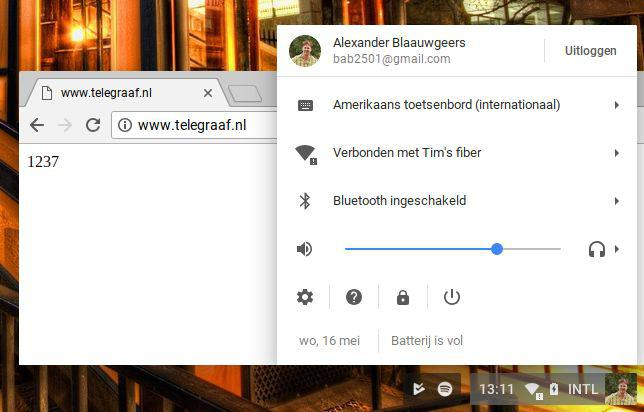
\includegraphics[width=\textwidth]{mitm.jpg}
\end{frame}


%----------------------------------------------------------------------------------
\section{Questions}
%----------------------------------------------------------------------------------

\begin{frame}{Questions?}

Questions?

%\def\newblock{}
%\bibliographystyle{unsrt}
%\bibliography{mybib}
\end{frame}

\end{document} 
%---------------------------------------------------------------------------
